\documentclass[a4paper,10pt]{article}
\usepackage[utf8]{inputenc}
\usepackage[MeX]{polski}
\usepackage{graphicx}
\usepackage{hyperref}
\usepackage{fancyvrb}

\title{[WEDT.A] Klasyfikacja typów serwisów WWW na postawie informacji o~strukturze strony i~tekstu}
\author{Michał Aniserowicz, Jakub Turek}
\date{}

\begin{document}

\maketitle

\section*{Opis problemu}

Zadanie polega na implementacji aplikacji, która dokonuje automatycznej klasyfikacji typów stron WWW na podstawie ich  struktury. Analiza może obejmować źródło strony, konfigurację rozmieszczenia komponentów (layout), a~także strukturę i~znaczenie zamieszczonych na stronie treści.

\section*{Założenia}

Projekt obejmuje implementację klasyfikatora następujących typów serwisów:

\begin{description}
 \item [Blog] rodzaj internetowego dziennika (pamiętnika), który zawiera odrębnie, chronologicznie uporządkowane wpisy. Przykład serwisu: \url{http://rafalstec.blox.pl/}.
 \item [Serwisy informacyjne] portale zawierające najnowsze wiadomości z~różnych dziedzin życia, takich jak polityka, finanse, technologie. Przykład serwisu: \url{http://onet.pl/}.
 \item [,,Kwejki''] serwisy społecznościowe oparte w~głównej mierze na grafikach. Przykład serwisu: \url{http://kwejk.pl/}.
 \item [Sklepy internetowe] portale umożliwiające zakup szerokiego asortymentu akcesoriów elektronicznych oraz komputerowych. Przykład serwisu: \url{http://wicomp.pl/}.
\end{description}

Dane wejściowe aplikacji stanowić będzie adres witryny internetowej. Na wyjście wyprowadzona zostanie nazwa kategorii lub informacja, że serwis nie został zaklasyfikowany do żadnej z~powyższych kategorii.

\begin{figure}[h!]
\centering
  \begin{Verbatim}[frame=single,baselinestretch=0.3]
<div class="tooltip-title-container">

  <div class="tooltip-title-left-corner">

    <div class="tooltip-title">

      <p class="tooltip-title-h2">

        <a href="/obrazek/1763501/autor-gry-o-tron.html">

          Autor Gry o Tron?

        </a>

      </p>

    </div>

    <div class="tooltip-title-right-corner"></div>

    <div class="clr"></div>

  </div>

</div>
  \end{Verbatim}
  \caption{Fragment kodu źródłowego witryny http://kwejk.pl.}
  \label{fig:kwejk_listing}
\end{figure}

\subsection*{Technologia}

Projekt zostanie zaimplementowany w~języku Python, przy wykorzystaniu wersji drugiej (2.7.4) interpretera języka. Implementacja będzie testowana w~środowiskach Windows oraz Unix (Ubuntu). Do implementacji zostaną wykorzystane standardowe moduły języka, między innymi:

\begin{description}
 \item[re] wyrażenia regularne,
 \item[htmllib] parser języka HTML.
\end{description}


\section*{Struktura danych}

Aplikacja umożliwiać będzie budowanie pełnego drzewa HTML. W~korzeniu drzewa przechowywane będą następujące informacje:

\begin{itemize}
 \item Typ napotkanego taga HTML, na przykład \verb+<div>+, \verb+<h1>+.
 \item Dodatkowe atrybuty taga powiązane z~CSS - kaskadowymi arkuszami styli: identyfikator \verb+id="_"+, klasa \verb+class="_"+ oraz styl elementu \verb+style="_"+.
 \item Tekst zawarty pomiędzy tagiem otwierającym a zamykającym. Przykładowo dla kodu \verb+<a>Odnośnik</a>+ jest to fraza ,,Odnośnik''.
 \item Inne atrybuty kontekstowe związane z~poszczególnymi tagami:
 
    \begin{itemize}
      \item dla obrazka (\verb+<img>+) - jego rozmiar oraz źródło pochodzenia (lokalne - z domeny, którą analizujemy lub zewnętrzne - spoza niej),
      \item dla nagłówków (\verb+<h1>+, \verb+<h2>+, itd.) - rozmiar czcionki.
    \end{itemize}
\end{itemize}

\begin{figure}[h!]
\centering
  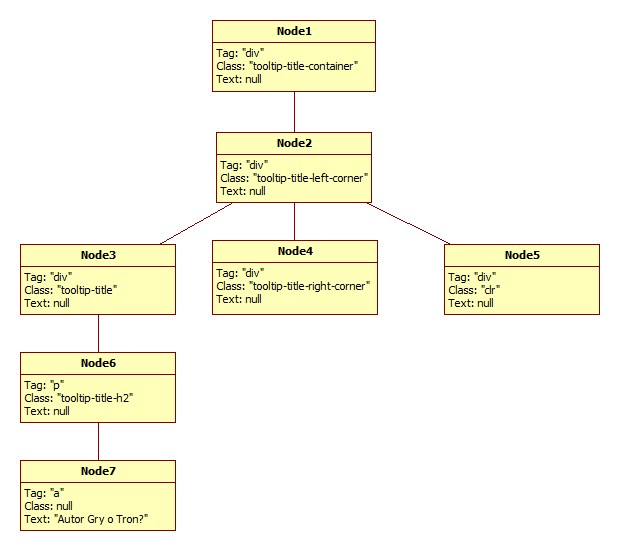
\includegraphics[width=.9\textwidth]{html_tree_full.jpg}
  \caption{Pełne drzewo HTML dla kodu przedstawionego na listingu \ref{fig:kwejk_listing}.}
  \label{fig:html_tree_full}
\end{figure}

Ze względu na rozmiary oraz skomplikowanie struktury dla dużych portali, takich jak sklepy internetowe lub serwisy informacyjne, kod aplikacji będzie udostępniał różne możliwości redukcji złożoności drzewa:

\begin{itemize}
 \item Zawężanie podzbioru tagów, dla których budowane jest drzewo. Tagi istotne dla struktury strony to, między innymi, \verb+<div>+, \verb+<td>+, \verb+<article>+, \verb+<h1>+, \verb+<a>+ oraz \verb+<img>+. Z~punktu widzenia zadania, tagi niosące niewiele informacji służą głównie do formatowania tekstu, jak na przykład \verb+<b>+, \verb+<span>+, oraz osadzania skryptów - \verb+<script>+.
 \item Ograniczanie stopnia zagnieżdżania korzeni w~drzewie:
    \begin{itemize}
	\item pomijanie węzłów przekraczających dany, parametryzowalny, poziom zagłębienia w~strukturze,
	\item sklejanie kilku następujących po sobie węzłów o~zbliżonych wymiarach na stronie w~jeden.
    \end{itemize}
 \item Odfiltrowywanie elementów uznanych za nieistotne metodami heurystycznymi, przykładowo prosty filtr eliminujący reklamy bazując na klasach obiektów.
\end{itemize}

\begin{figure}[h!]
\centering
  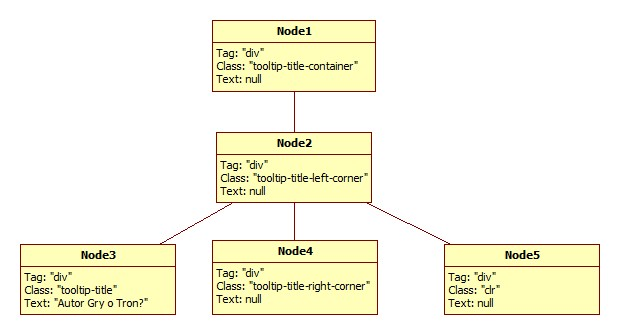
\includegraphics[width=.9\textwidth]{html_tree_cropped.jpg}
  \caption{Drzewo HTML z~rysunku \ref{fig:html_tree_full} zredukowane do tagów div.}
  \label{fig:html_tree_cropped}
\end{figure}

\section*{Algorytm}
\subsection*{Blogi}

Algorytm kategoryzacji blogów będzie rozpoznawał dzienniki internetowe w~dwukolumnowym układzie. W~szerszej kolumnie znajdują się notki, natomiast węższa kolumna to menu strony. Notki posiadają pewną stałą strukturę wewnętrzną. Na pojedynczy wpis składają się: tytuł, treść, data, informacja o~autorze oraz link do komentarzy. Menu charakteryzuje się natomiast występowaniem dużej ilości podobnych odnośników jeden pod drugim (archiwum dla kolejnych miesięcy, kategorie wpisów, odnośniki do zaprzyjaźnionych blogów). Szablon bloga przedstawia rysunek \ref{fig:blog_template}. Przykłady stron o~takiej strukturze przedstawiono na rysunkach \ref{fig:blog_scott} oraz \ref{fig:blog_simon}.

\begin{figure}[h!]
\centering
  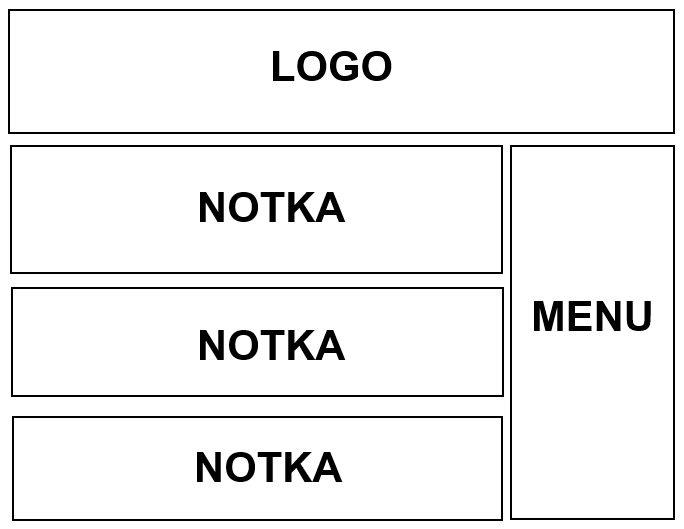
\includegraphics[width=.5\textwidth]{blog_template.png}
  \caption{Szablon, na którym oparta jest większość współczesnych blogów.}
  \label{fig:blog_template}
\end{figure}

\begin{figure}[h!]
\centering
  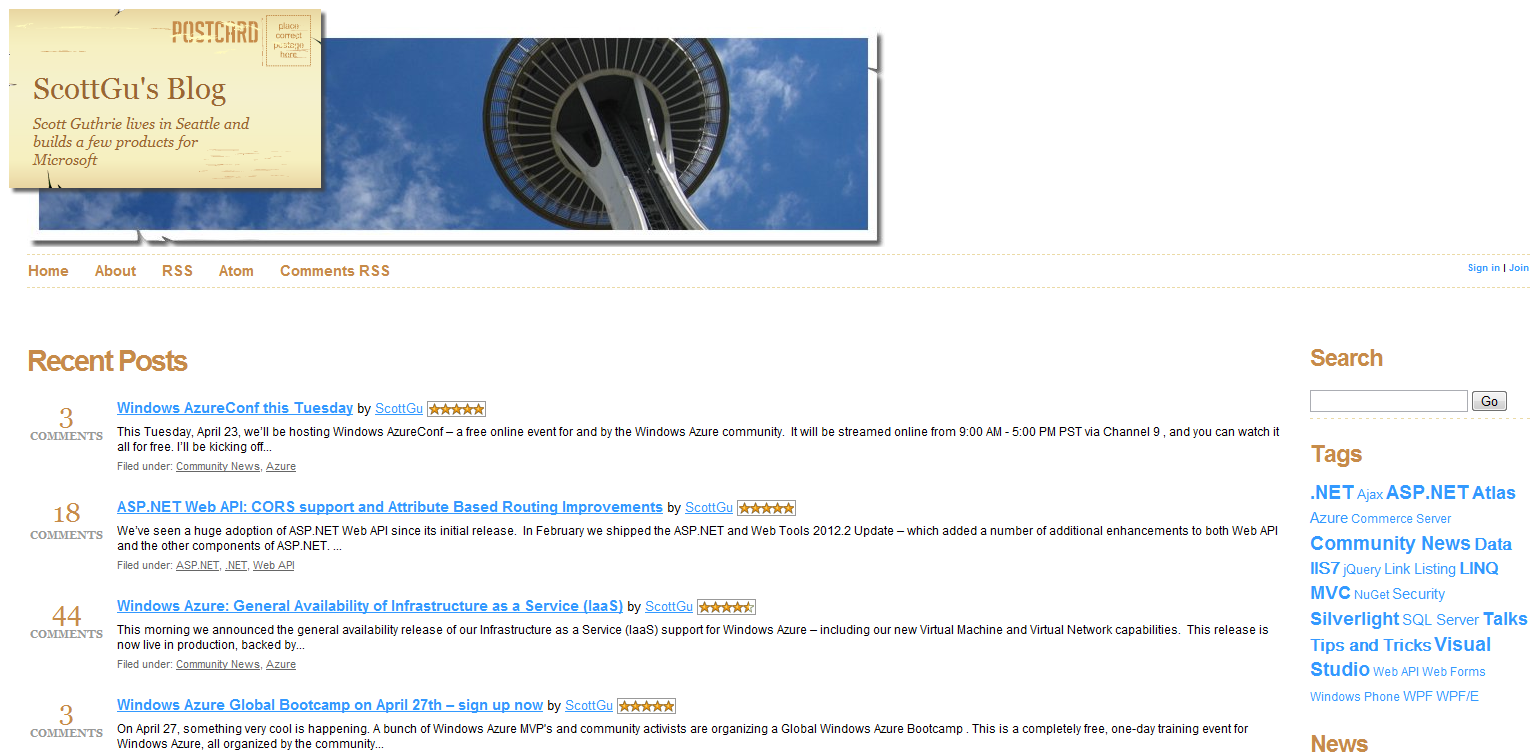
\includegraphics[width=.9\textwidth]{blog_scott.png}
  \caption{Przykład dwukolumnowej struktury bloga.}
  \label{fig:blog_scott}
\end{figure}

\begin{figure}[h!]
\centering
  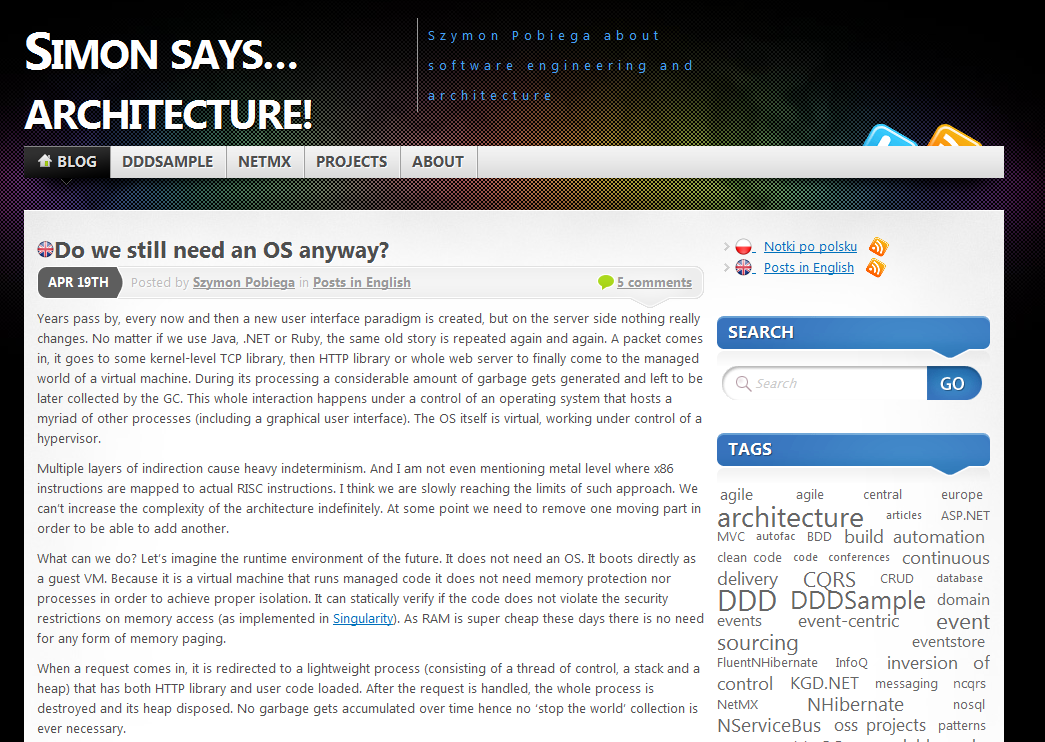
\includegraphics[width=.9\textwidth]{blog_simon.png}
  \caption{Przykład dwukolumnowej struktury bloga.}
  \label{fig:blog_simon}
\end{figure}

Algorytm rozpoznawania blogów będzie działał według następującego schematu:

\begin{enumerate}
 \item Odnalezienie w~drzewie powtarzającego się układu węzłów, które reprezentują notkę. Cechy charakterystyczne takiego układu to:
    \begin{itemize}
     \item Duża ilość tekstu zawartego pomiędzy tagami strukturalnymi, z~niewielką ilością odnośników.
     \item Można wyróżnić przynajmniej tytuł notki oraz odnośnik do komentarzy.
     \item Odpowiadające tagi strukturalne mają identyczne właściwości - klasy kaskadowych arkuszy styli.
     \item Kolejne struktury umieszczone są w~kodzie jedna pod drugą oraz wszystkie mają wspólnego rodzica.
     \item Powtarzalność struktury wynosi co najmniej pięć (założenie heurystyczne).
    \end{itemize}
  \item Odnalezienie w~drzewie układu węzłów, który repreprezentuje menu strony (schematyczne odnośniki występujące jeden pod drugim i~prowadzące głównie do adresów w~domenie lokalnej - archiwum oraz kategorie).
  \item Badanie wzajemnych pozycji odnalezionych kolumn - powinny być umieszczone horyzontalnie względem siebie.
  \item Odnalezienie nagłówka strony, czyli największego elementu graficznego / tekstowego na stronie, występującego pojedynczo. 
  \item Badanie wzajemnych pozycji przypuszczalnego nagłówka strony oraz kolumn zawierających menu i~wpisy. Nagłówek strony musi znajdować się ponad pozostałymi kolumnami.
\end{enumerate}

\noindent Jeżeli wszystkie elementy udało się odnaleźć oraz spełnione są przytoczone założenia przestrzenne, to witryna kategoryzowana jest jako blog.

\subsection*{Strony informacyjne}

Strony informacyjne charakteryzują się liczną zawartością odnośników w~domenie lokalnej. Podobnie jak w~przypadku blogów, dominuje układ dwukolumnowy, przy czym kolumna szersza jest zazwyczaj nieustrukturalizowana, natomiast kolumna węższa zawiera wiele odnośników jeden pod drugim. Logotyp nie jest dominującym elementem strony i~ciężko wyznaczyć go na bazie wielkości, zazwyczaj położony jest w~lewym górnym rogu witryny. Ponadto, strony informacyjne charakteryzują się wykorzystaniem trzypoziomowej strukturyzacji oferowanej przez HTML5, za pomocą tagów \verb+<div>+, \verb+<article>+ oraz \verb+<section>+.

Algorytm rozpoznawania stron informacyjnych będzie działał według następującego schematu:

\begin{enumerate}
 \item Zbadanie proporcji zwykłego tekstu występującego w~ramach odnośników (\verb+<a>...</a>+) oraz innych tagów zawierających tekst widoczny na witrynie.
 \item Określenie częstotliwości wykorzystania tagów \verb+<article>+ oraz \verb+<span>+ do strukturyzacji zagnieżdzonych odnośników do domen lokalnych (newsy).
 \item Odnalezienie wąskiej kolumny zawierającej odnośniki do wiadomości.
\end{enumerate}

Jeżeli proporcje w~punkcie 1. są $\gg 1$ oraz częstotliwość w~punkcie 2. jest wysoka, a~także udało odnaleźć się kolumnę z~punktu 3. to strona klasyfikowana jest jako strona informacyjna.

\subsection*{,,Kwejki''}

Strony typu \emph{kwejk} charakteryzują się występowaniem pojedynczej, centralnej kolumny, która zawiera dużych rozmiarów obrazy umieszczone jeden pod drugim. Obrazy te są najczęściej prezentowane w~ramach jednego ,,pudełka'', a~więc są osadzone w~regularnej strukturze tagów HTML. Ponad obrazami znajduje się logotyp oraz menu strony, natomiast pod nimi umieszczone jest małe menu nawigacyjne, prezentujące kolejne liczby (strony). Ogólny szablon stron typu \emph{kwejk} przedstawia rysunek \ref{fig:image_meme_template}, natomiast rysunki \ref{fig:image_meme_kwejk} oraz \ref{fig:image_meme_demotywatory} pokazują przykłady takich stron.

\begin{figure}[h!]
\centering
  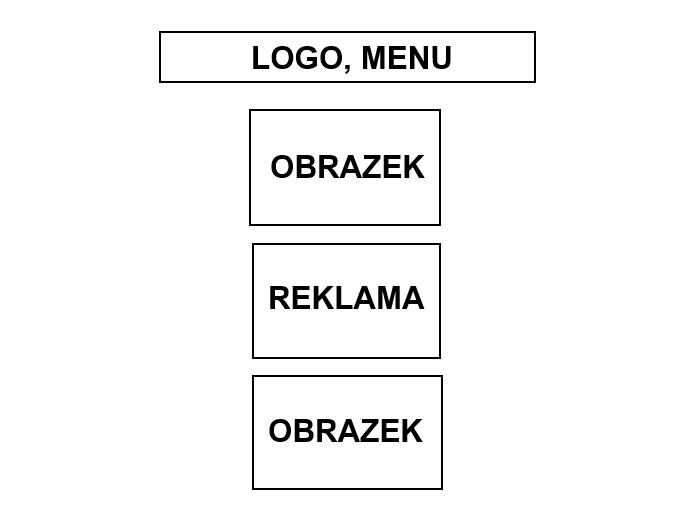
\includegraphics[width=.5\textwidth]{image_meme_template.png}
  \caption{Szablon stron typu \emph{kwejk}.}
  \label{fig:image_meme_template}
\end{figure}

\begin{figure}[h!]
\centering
  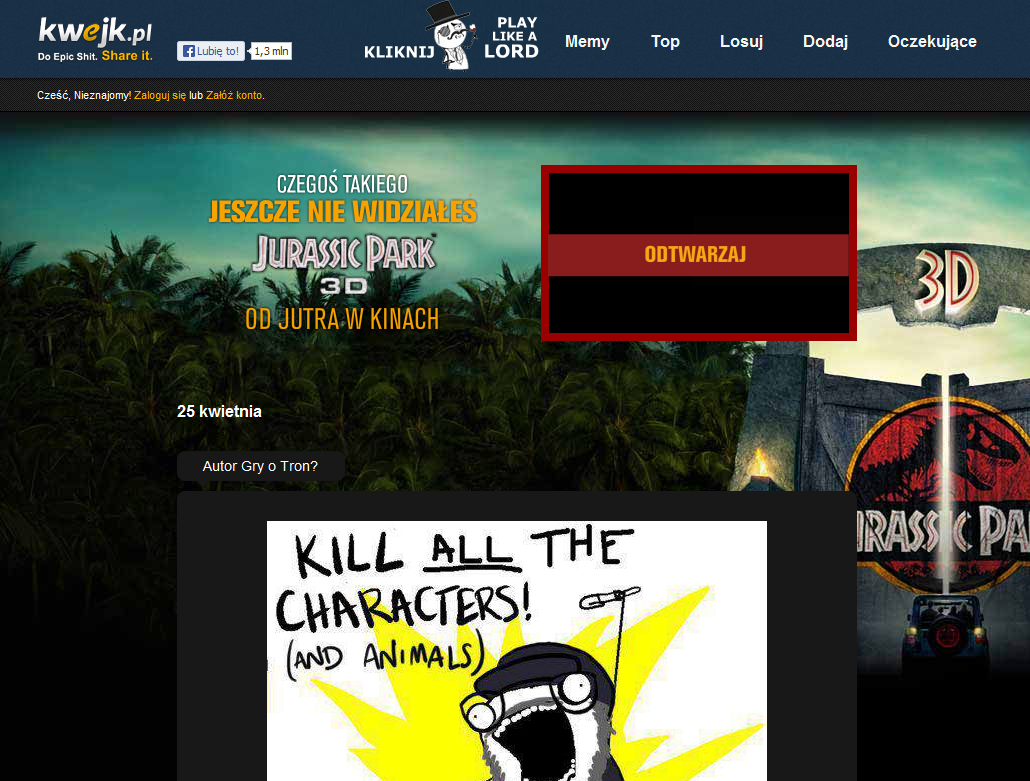
\includegraphics[width=.9\textwidth]{image_meme_kwejk.png}
  \caption{Portal społecznościowy http://kwejk.pl oparty na grafikach.}
  \label{fig:image_meme_kwejk}
\end{figure}

\begin{figure}[h!]
\centering
  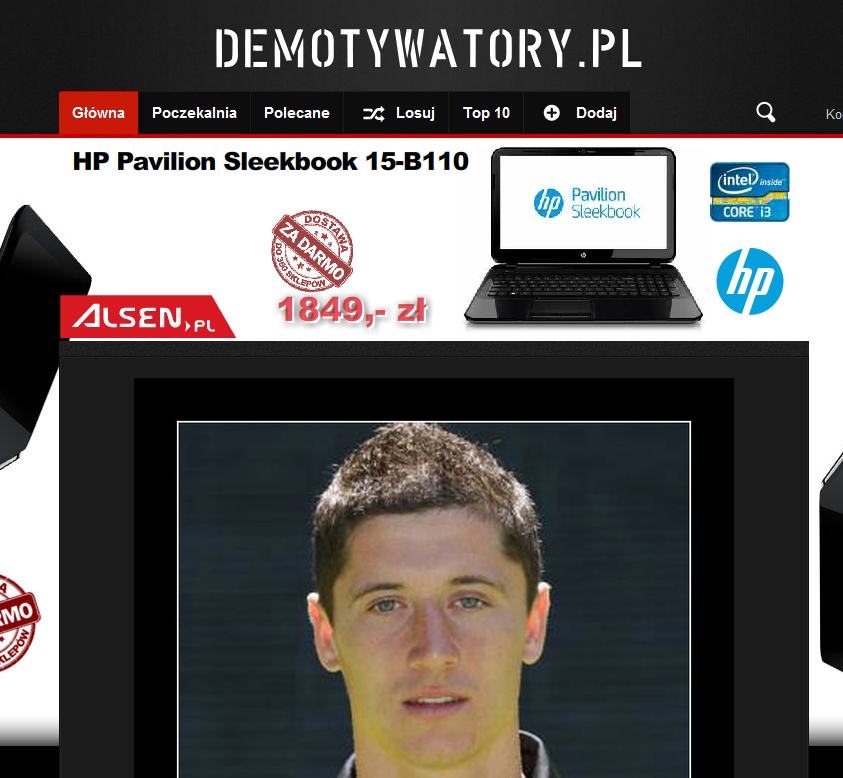
\includegraphics[width=.9\textwidth]{image_meme_demotywatory.png}
  \caption{Portal społecznościowy http://demotywatory.pl oparty na grafikach.}
  \label{fig:image_meme_demotywatory}
\end{figure}

Algorytm kategoryzacji ,,kwejków'' polega na odnalezieniu powtarzającej się struktury węzłów, o wspólnym rodzicu i~identycznych właściwościach, w~każdym z których osadzona jest pojedyncza grafika. Jeżeli taka struktura występuje, badane jest położenie tej struktury na stronie. W~przypadku, gdy kolumna jest wyśrodkowana, strona może zostać zakwalifikowana jako ,,kwejk''.

\subsection*{Sklepy internetowe}

Strony sklepów komputerowych lub ze sprzętem elektronicznym charakteryzują się \emph{kafelkowym} ułożeniem głównej części witryny. Każdy \emph{kafelek} odpowiada specyficznej kategorii towaru, jest ozdobiony pojedynczą grafiką i~zawiera wiele odnośników do stron w~domenie lokalnej, które odpowiadają podkategoriom produktów. Cechą charakterystyczną jest również zwielokrotniona nawigacja obejmująca:

\begin{itemize}
 \item klasyczne menu po lewej lub prawej stronie,
 \item dwa paski nawigacyjne umieszczone bezpośrednio nad i~pod \emph{kafelkami},
 \item menu z~tabularyczną strukturą linków znajdujące się w~stopce strony.
\end{itemize}

\noindent Istotnym elementem układu strony jest również duży logotyp sklepu, umieszczony w~górej części strony. 

Algorytm klasyfikacji sklepów internetowych oparty będzie na poszukiwaniu \emph{kafelków}. Do ich odnalezienia wykorzystane zostanie poszukiwanie regularnej struktury w~drzewie, o~następującej charakterystyce:

\begin{itemize}
 \item identyczne klasy elementów rozmieszczonych w~układzie tabelarycznym,
 \item każdy element zawiera niewielkich rozmiarów grafikę,
 \item każda kategoria opisana jest promocyjnym towarem - wyszukiwanie wzorca regularnego \verb+<kwota> <waluta>+ w~tekście.
\end{itemize}

\section*{Testowanie}

Testy opierać się będą na wykorzystaniu gotowego zestawu wstępnie skategoryzowanych witryn. Program testowy, dla każdej strony w~zbiorze, wywoła aplikację kategoryzującą i~na podstawie danych oceni, czy witryna została przydzielona do prawidłowej grupy. Na tej podstawie zostanie obliczona procentowa skuteczność każdego z~algorytmów kategoryzacji. Zbiór witryn testowych dobierany będzie według następujących kryteriów:

\begin{itemize}
 \item Reprezentatywny (liczący przynajmniej 100 elementów) zbiór próbek dla każdej z~kategorii.
 \item W~ramach każdego zestawu występują strony w~przynajmniej trzech różnych językach naturalnych.
 \item Dodatkowy, liczny zbiór witryn, których nie można przydzielić do żadnej z~kategorii.
\end{itemize}

\noindent Przykładowe, niepełne listy skategoryzowanych witryn zostały dołączone do dokumentacji.

Dla każdego z~algorytmów zostaną wyznaczone następujące zbiory:

\begin{itemize}
 \item $TP$ (true positives) - poprawne przydzielenie witryny do kategorii (algorytm wskazał, że witryna należy do kategorii, gdy w~rzeczywistości do niej należy),
 \item $TN$ (true negatives) - poprawne nieprzydzielenie witryny do kategorii (algorytm wskazał, że witryna nie należy do kategorii, gdy w~rzeczywistości do niej nie należy),
 \item $FP$ (false positives) - błędne przydzelenie witryny do kategorii (algorytm wskazał, że witryna należy do kategorii, gdy w~rzeczywistości do niej nie należy),
 \item $FN$ (false negatives) - błędne nieprzydzielenie witryny do kategorii (algorytm wskazał, że witryna nie należy do żadnej kategorii, gdy w~rzeczywistości do niej należy).
\end{itemize}

\noindent Na podstawie tych wartości, dla każdego algorytmu zostaną wyznaczone:

\begin{itemize}
 \item precyzja - $\frac{|TP|}{|TP| + |FP|}$,
 \item zupełność - $\frac{|TP|}{|TP| + |FN|}$,
 \item dokładność - $\frac{|TP| + |TN|}{|TP| + |TN| + |FP| + |FN|}$,
 \item zaszumienie - $\frac{|FP|}{|FP| + |TN|}$.
\end{itemize}

\end{document}